\label{sec:correlation}

\section{Correlation Matrices for backgrounds in BDTs}

\newpage 

\begin{figure}[H]
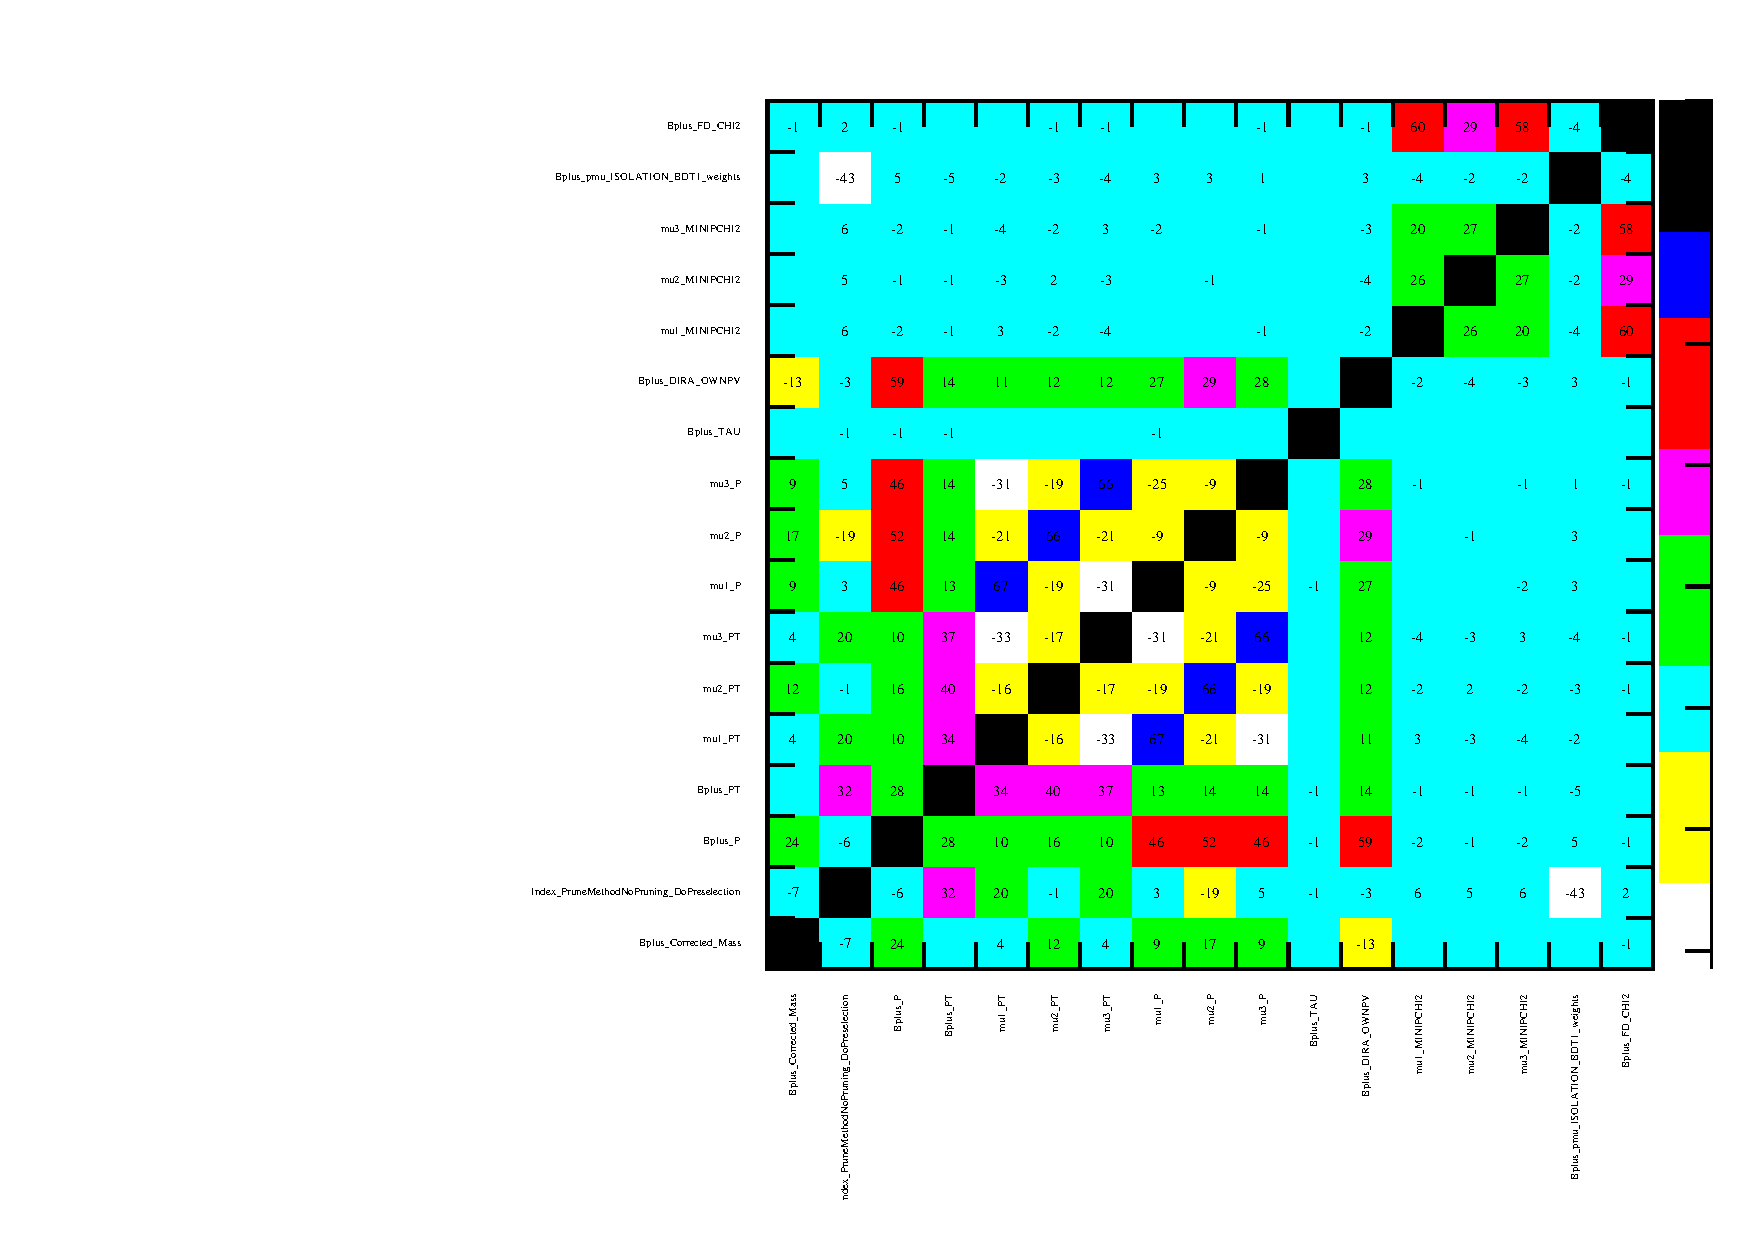
\includegraphics[width=0.6\linewidth]{./figs/appendix/CorrelationBDTvarsbkgMCSig2012_vs_DATACombiRun1.pdf}\put(-50,133){(a)}
\newline 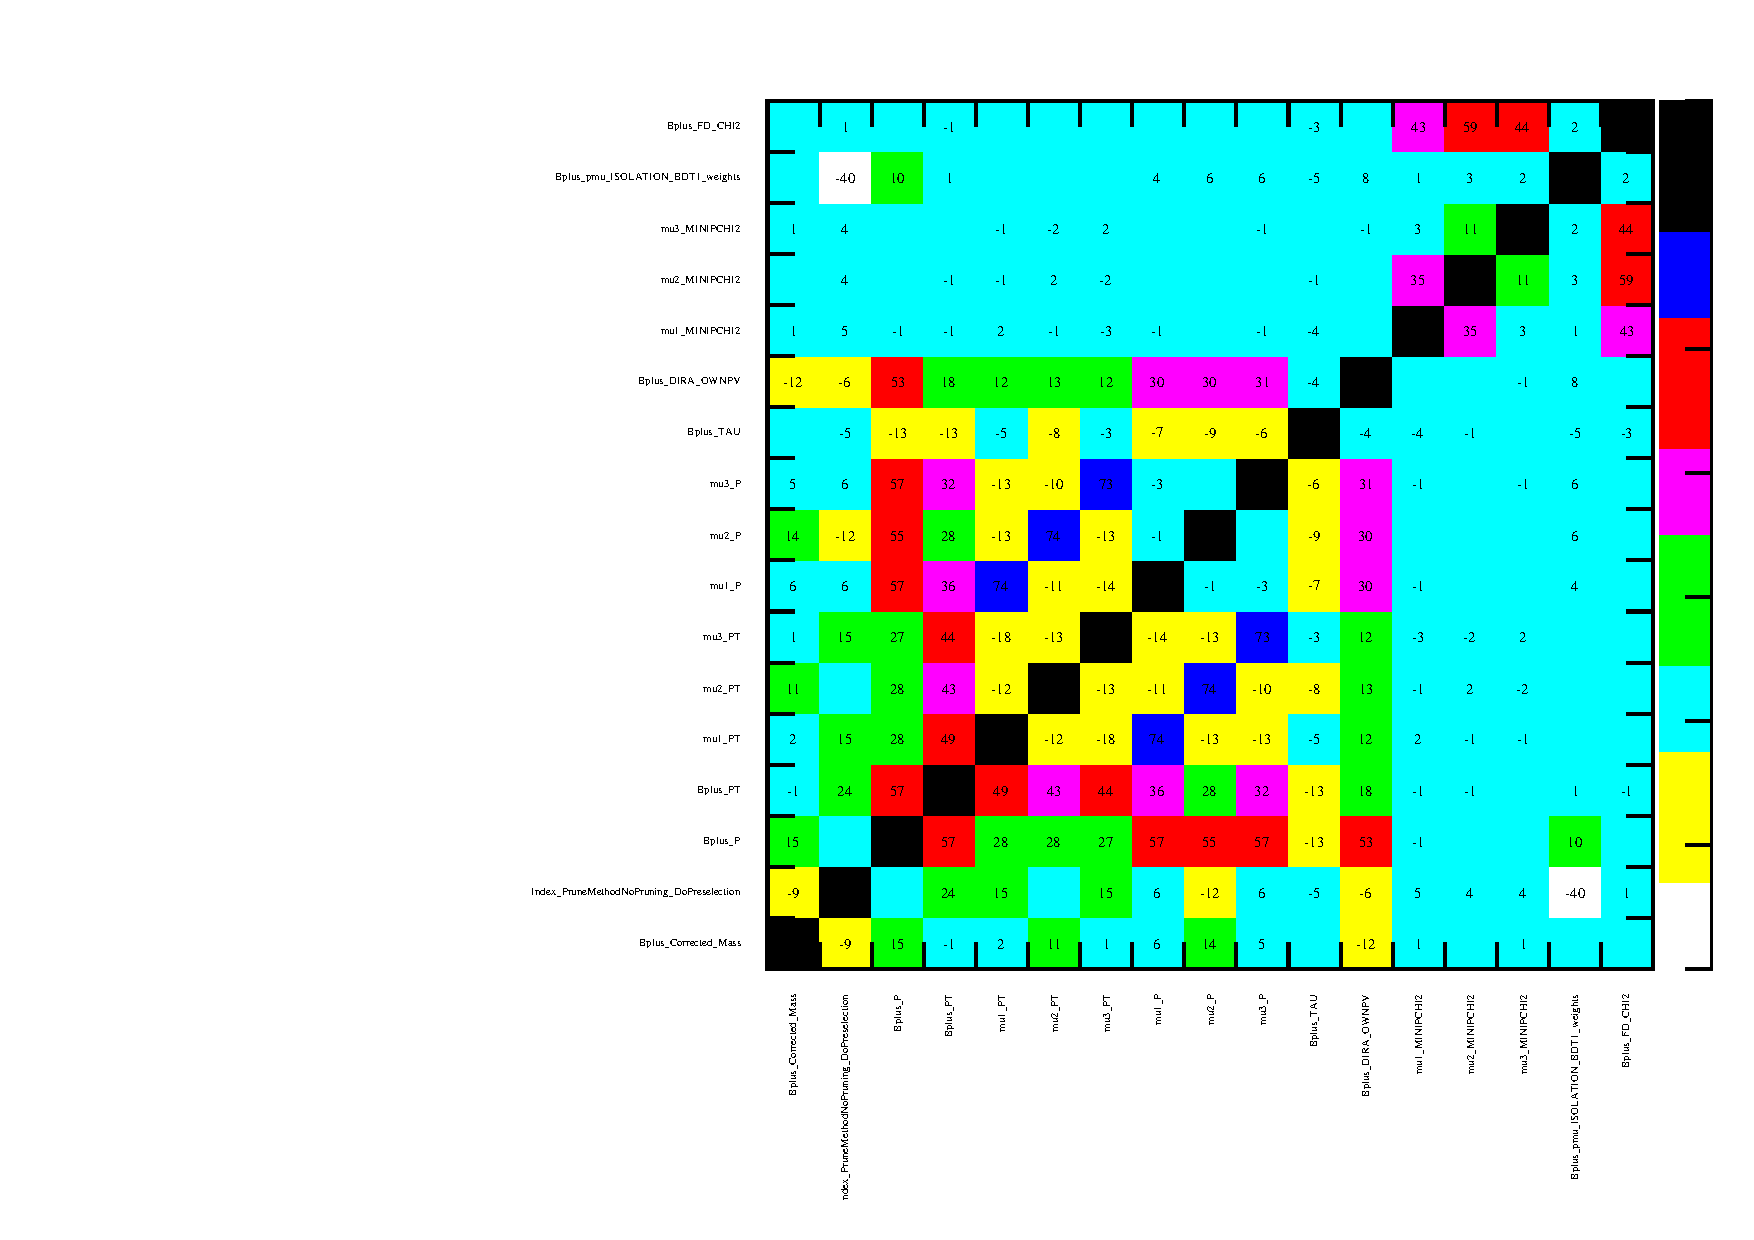
\includegraphics[width=0.6\linewidth]{./figs/appendix/CorrelationBDTvarsbkgMCSig2016_288888335_vs_DATACombi2016.pdf}\put(-50,133){(b)}
	\caption{Correlation matrix for all input variables, corrected mass as well resulting BDT variable for both (a) Run \Rn{1} Combinatorial BDT (b) 2016 Combinatorial BDT for background sample.}
\label{fig:correlationcombi}
\end{figure}


\begin{figure}[H]
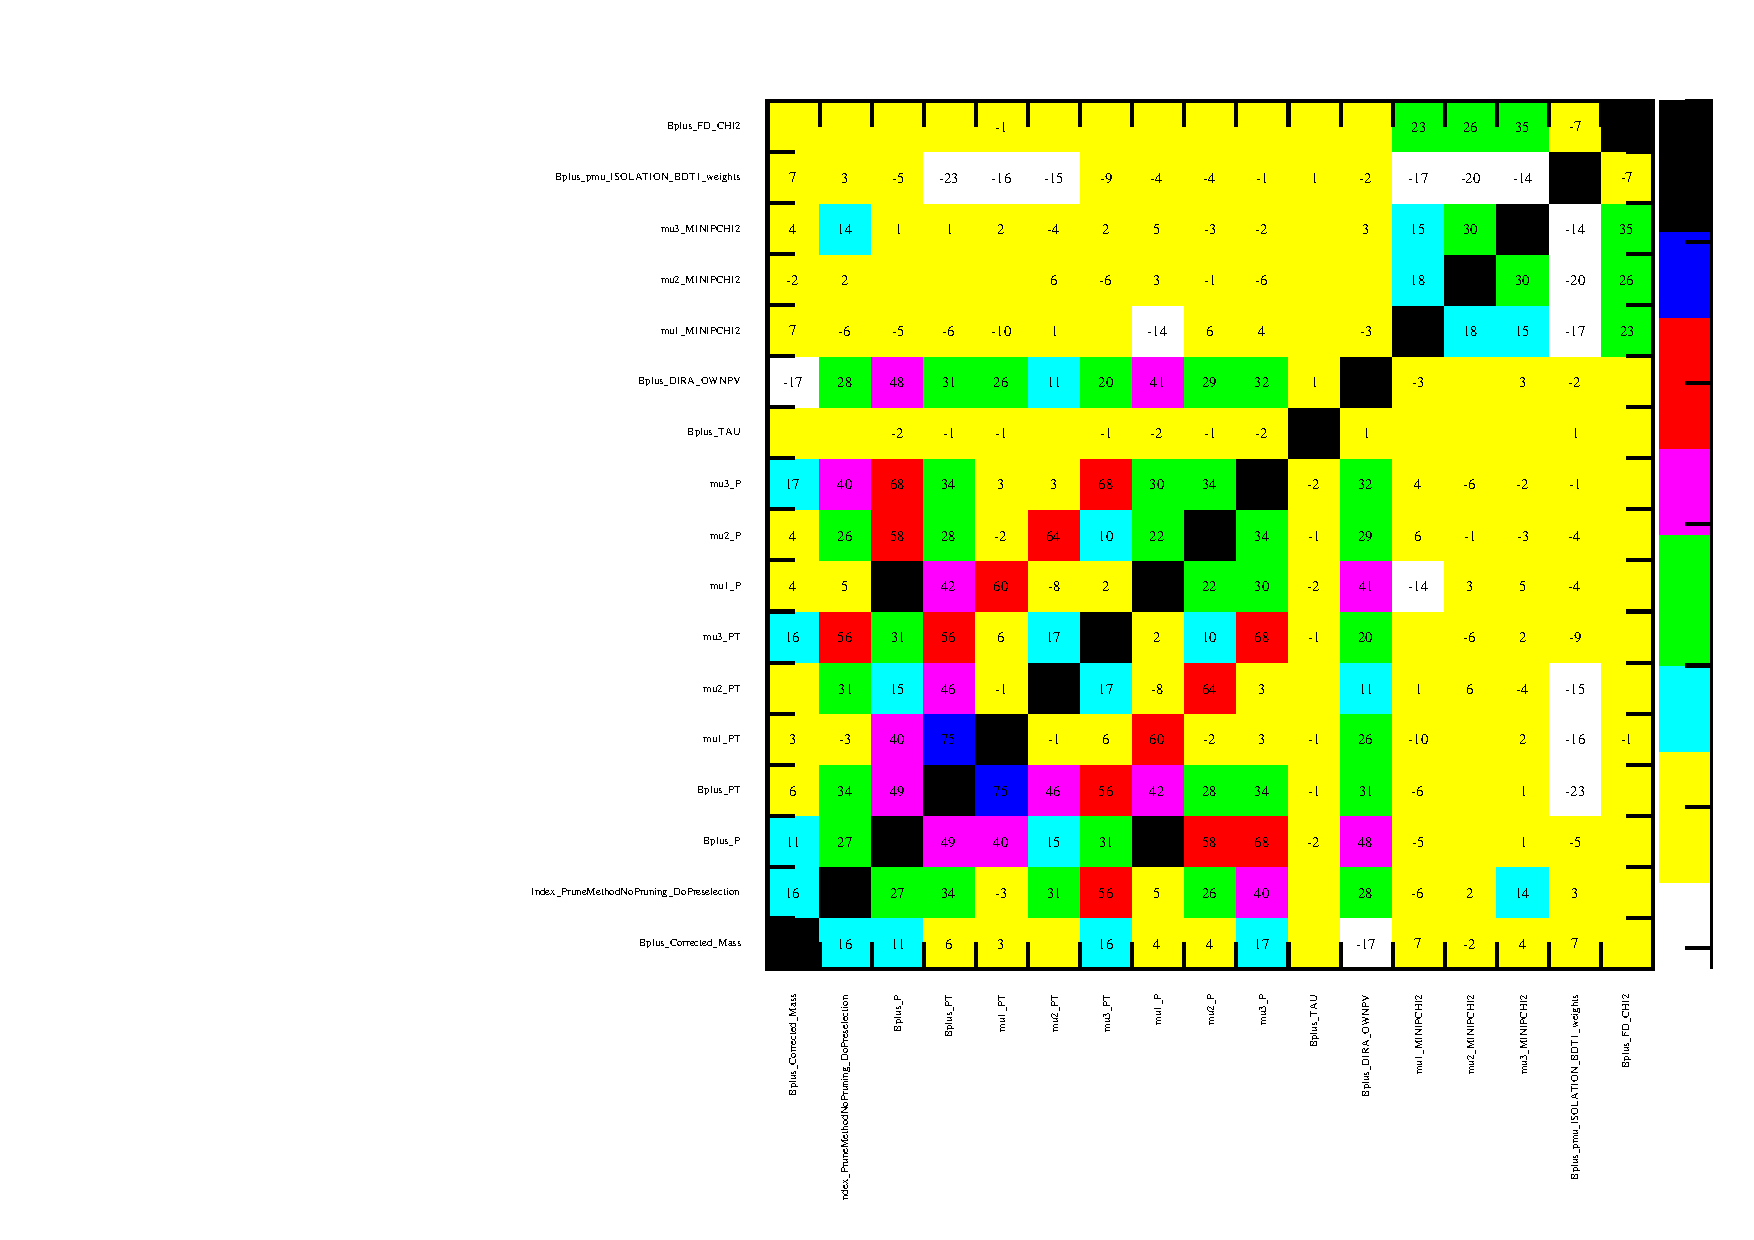
\includegraphics[width=0.6\linewidth]{./figs/appendix/CorrelationBDTvarsbkgMCSig2012_vs_DATAMisidRun1.pdf}\put(-50,133){(a)}
\newline 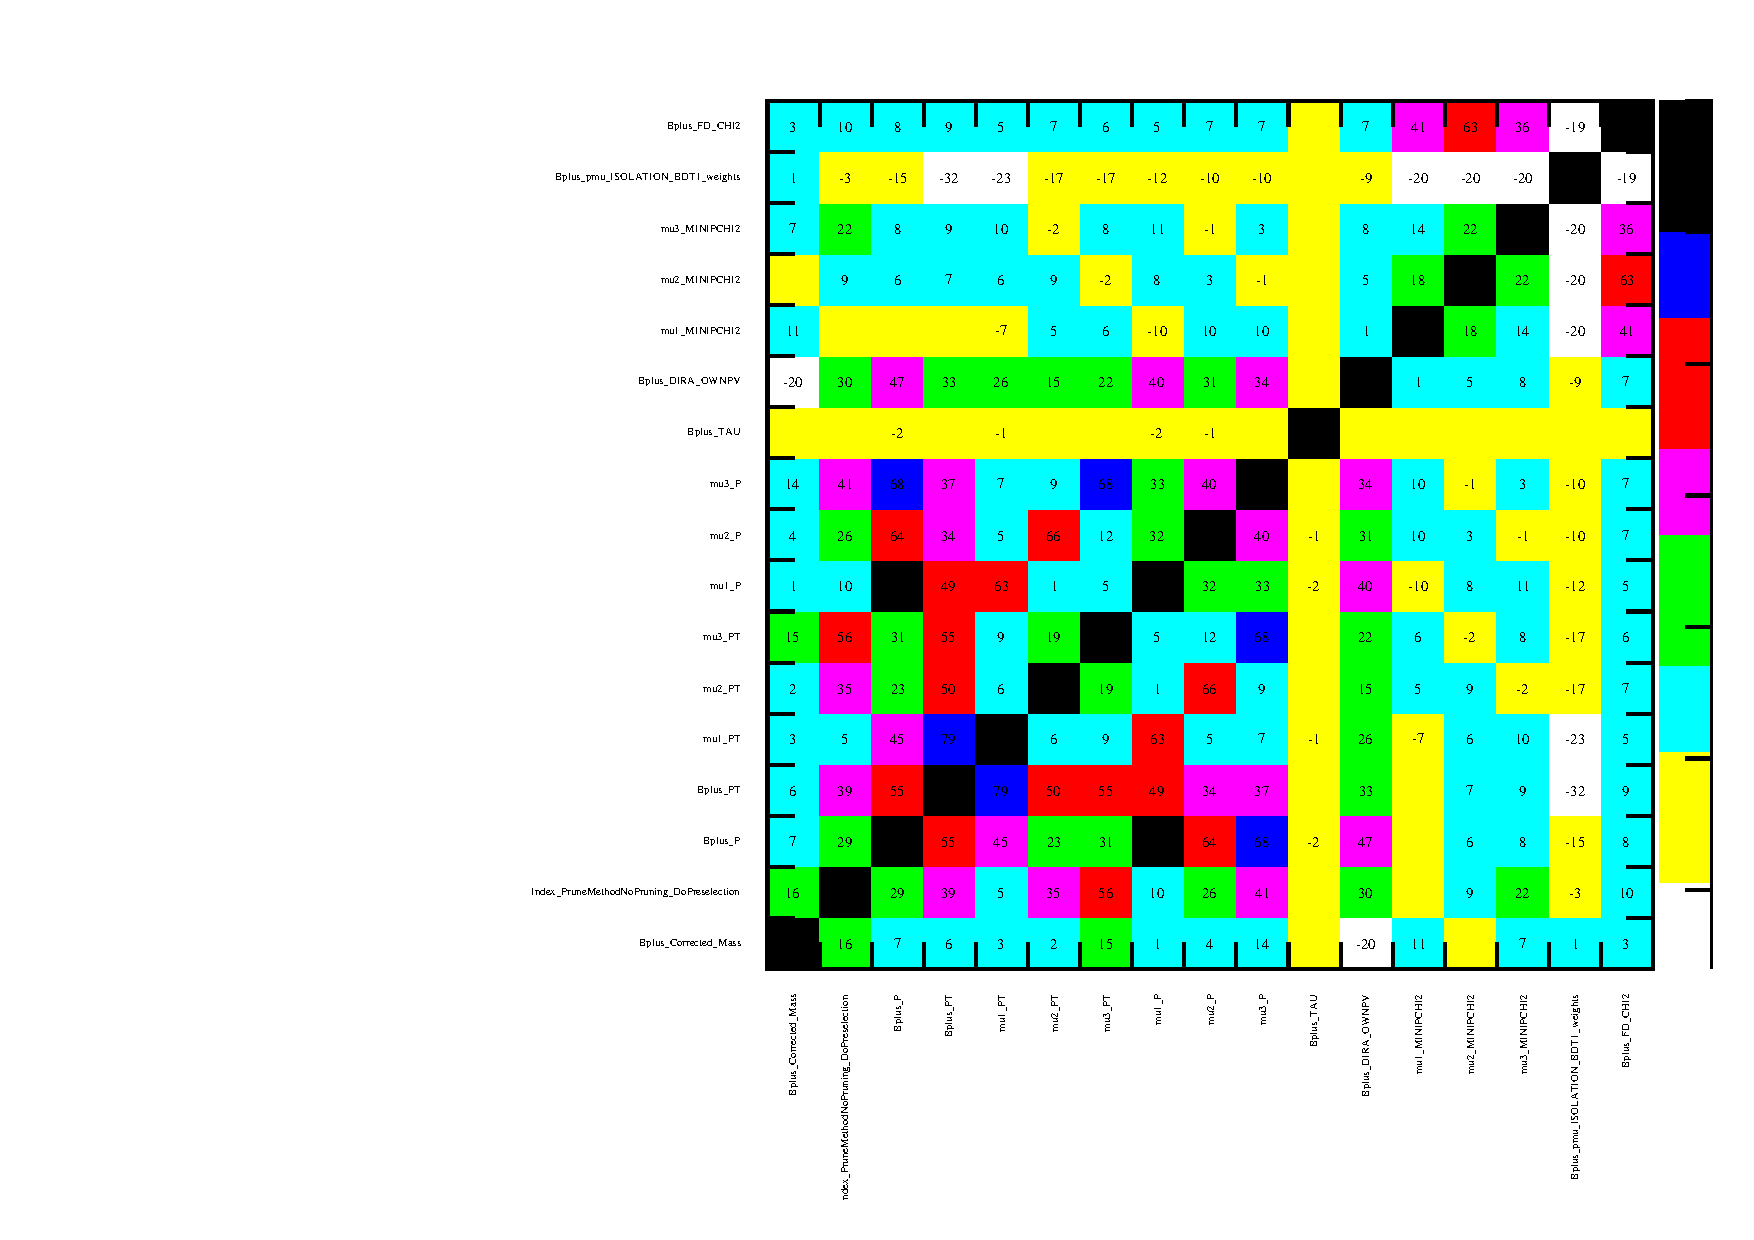
\includegraphics[width=0.6\linewidth]{./figs/appendix/CorrelationBDTvarsbkgMCSig2016_288888335_vs_DATAMisid2016.pdf}\put(-50,133){(b)}
	\caption{Correlation matrix for all input variables, corrected mass as well resulting BDT variable for both (a) Run \Rn{1} Misid BDT (b) 2016 Misid BDT for background sample.}
\label{fig:correlationmisid}
\end{figure}

